\documentclass{article}

\usepackage{graphicx}
\usepackage{tikz}
\usepackage{tikzsymbols}
\usetikzlibrary{calc,patterns,shapes.geometric}
\pagestyle{empty}
\usepackage[margin=0pt]{geometry}
\geometry{papersize={14in,12in}}

\def\centerarc[#1](#2)(#3:#4:#5){\draw[#1] ($(#2)+({#5*cos(#3)},{#5*sin(#3)})$) arc (#3:#4:#5);}

\begin{document}
	\begin{figure}
		\centering
		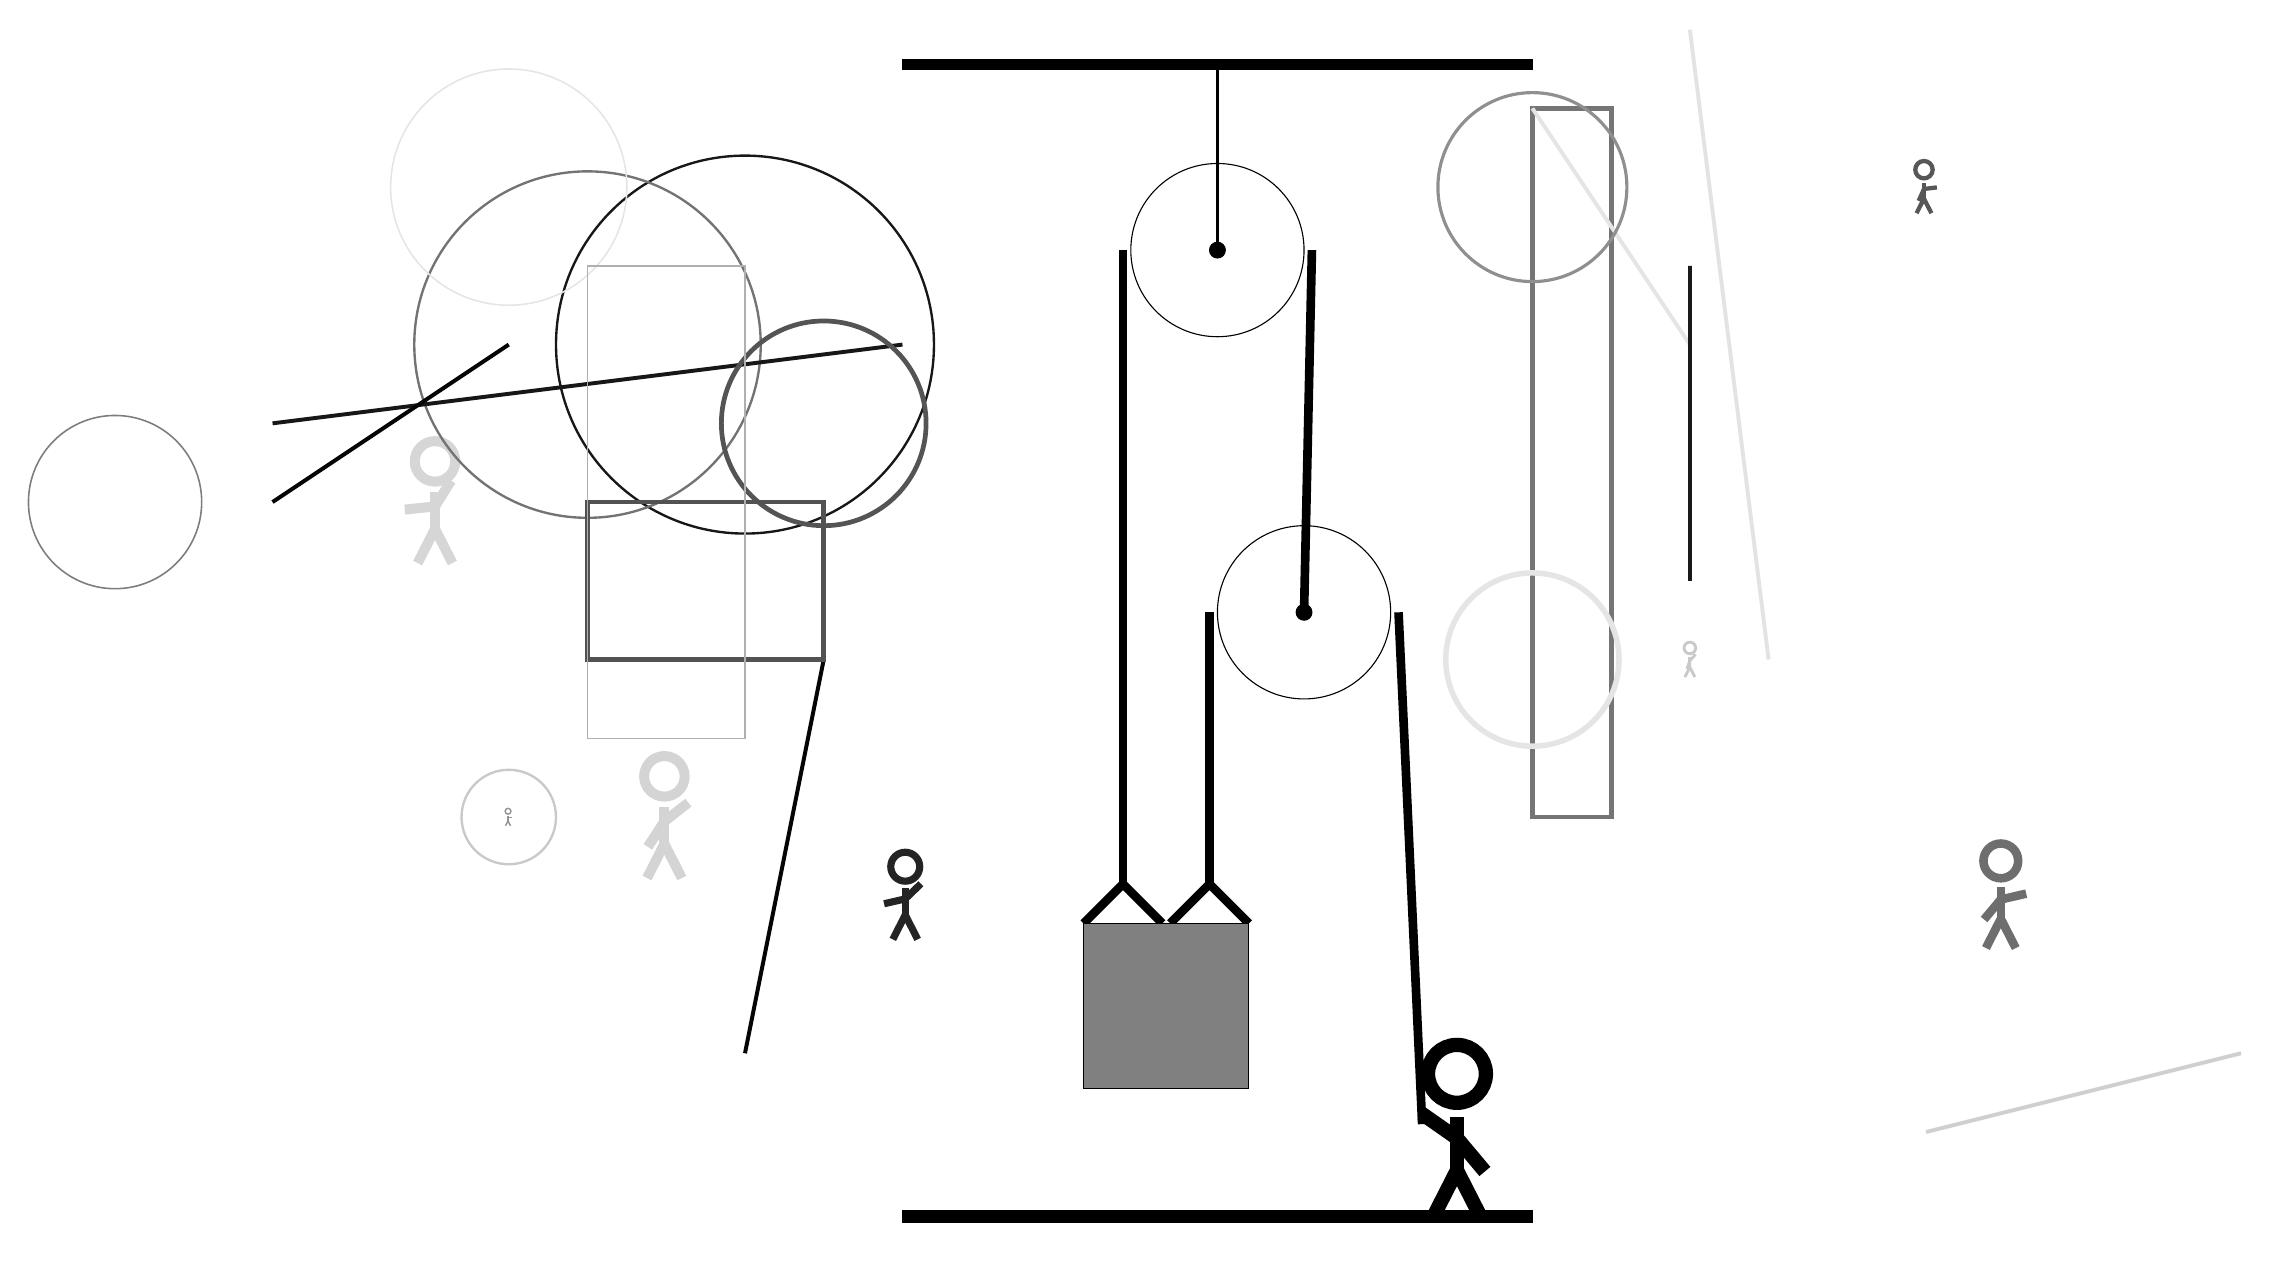
\begin{tikzpicture}
			%%%%% START %%%%%
			
			\draw[fill=black] (-2, 11.5) rectangle (6, 11.625);
			
			\draw (2, 9.2) circle (1.1);
			\draw[fill=black] (2, 9.2) circle (0.1);
			\draw[thick] (2, 9.2) -- (2, 11.5);
			
			\draw (3.1, 4.6) circle (1.1);
			\draw[fill=black] (3.1, 4.6) circle (0.1);
			
			\draw[line width = 1.1mm]  (0.3, 0.65) -- (0.8, 1.15) -- (1.3, 0.65);
			\draw[line width = 1.1mm]  (1.4, 0.65) -- (1.9, 1.15) -- (2.4, 0.65);
			\draw[fill=black!50] (0.3, 0.65) rectangle (2.4, -1.45);
			
			\draw[line width = 1.1mm] (0.8, 9.2) -- (0.8, 1.15);
			\centerarc[line width = 1.1mm](2, 9.2)(0:180:1.2000000000000002);
			\draw[line width = 1.1mm] (3.2, 9.2) -- (3.1, 4.6);
			\draw[line width = 1.1mm] (1.9, 4.6) -- (1.9, 1.15);
			\centerarc[line width = 1.1mm](3.1, 4.6)(0:180:1.2000000000000002);
			\draw[line width = 1.1mm] (4.3, 4.6) -- (4.6, -1.9);
			
			\node[line width=0.3mm, color=black!57] at (12, 1) {\Strichmaxerl[6][50][13]};
			
			\draw[line width=0.6mm, color=black!54] (7, 11) rectangle (6, 2);
			\draw [line width=0.2mm, color=black!51](-12, 6) circle (1.1);
			\draw[line width=0.5mm, color=black!19](11, -2) -- (15, -1);
			\node[line width=0.7mm, color=black!16] at (-8, 6) {\Strichmaxerl[7][6][58]};
			\node[line width=0.2mm, color=black!66] at (11, 10) {\Strichmaxerl[3][66][7]};
			\draw [line width=0.3mm, color=black!91](-4, 8) circle (2.4);
			\draw[line width=0.5mm, color=black!11](8, 12) -- (9, 4);
			\draw[line width=0.5mm, color=black!10](8, 8) -- (6, 11);
			
			\draw [line width=0.3mm, color=black!55](-6, 8) circle (2.2);
			\node[line width=0.4mm, color=black!42] at (-7, 2) {\Strichmaxerl[1][85][0]};
			
			\draw[line width=0.5mm, color=black!90] (8, 5) rectangle (8, 9);
			\draw[line width=0.5mm, color=black!91](-2, 8) -- (-10, 7);
			
			\draw [line width=0.4mm, color=black!44](6, 10) circle (1.2);
			\draw[line width=0.5mm, color=black!98](-4, -1) -- (-3, 4);
			\node[line width=0.2mm, color=black!21] at (8, 4) {\Strichmaxerl[2][70][49]};
			
			\node[line width=0.5mm, color=black!17] at (-5, 2) {\Strichmaxerl[7][57][38]};
			
			\draw [line width=0.2mm, color=black!10](-7, 10) circle (1.5);
			\draw [line width=0.6mm, color=black!67](-3, 7) circle (1.3);
			\draw [line width=0.7mm, color=black!10](6, 4) circle (1.1);
			\node[line width=0.4mm, color=black!86] at (-2, 1) {\Strichmaxerl[5][13][44]};
			
			\draw[line width=0.5mm, color=black!98](-7, 8) -- (-10, 6);
			\draw[line width=0.6mm, color=black!68] (-3, 4) rectangle (-6, 6);
			\draw [line width=0.3mm, color=black!21](-7, 2) circle (0.6);
			\draw[line width=0.2mm, color=black!31] (-4, 3) rectangle (-6, 9);
			
			
			\node at (5, -2) {\Strichmaxerl[10][-35][-50]};
			
			\draw[fill=black] (-2, -3) rectangle (6, -3.15);
			
			%%%%% END %%%%%
		\end{tikzpicture}
	\end{figure}	
\end{document}